\section{Graph colorings and rainbow Schur triples: statements, provenance, and proofs}
\label{app:structural-case-studies}
\label{sec:counterexample-structure}
This appendix states the two family theorems of Section~\ref{sec:mathematics} in full, records where their witnesses and certificates come from, and proves them. Both witnesses refute published conjectures. They were found on 4 September 2026 by \texttt{gpt-5.6-sol} at maximum reasoning effort, in runs that asked the model to prove or refute the statements without access to BugBank, and were accepted by separate model checks. They entered the research-discovery collection on 10 September, apart from the 285-dossier construction stage and the human-approved core. The Schur witness already supplied an infinite family with exact counts, and the follow-up optimizes the larger two-threshold family it belongs to and measures the loss from moving the thresholds. The graph witness was one cycle blowup, and the follow-up classifies the odd cycle lengths and counts all frozen six-colorings. We developed the family theorems and their proofs with the help of AI tools, and report them separately from the benchmark's dossier and input counts.

\paragraph{Graph certificates.}
Three theorems cover the original witness, the refutation of the source conjecture, and the family. The file \path{mathematics/supporting/sources/C9K2_frozen_coloring.lean} defines the adjacency of $C_9[K_2]$ and explicit five- and six-colorings; its theorem \path{C9K2.frozen_six_colouring_certificate} checks a proper six-coloring in which no vertex can change color, a proper coloring with at most five colors, and a second proper six-coloring, so the first six-coloring is isolated although another proper six-coloring exists. The theorem \texttt{Recol.not\_conjecture1} in \path{mathematics/supporting/sources/PrimeBlowup.lean} supplies what a refutation of the conjecture needs beyond the obstruction: it checks that $C_9$ satisfies the conjecture's hypotheses, using a degeneracy lemma~\citep{cereceda2008connectedness} that covers arbitrarily many colors and shows every induced subgraph of $C_9$ recolorable, and it refutes the conjecture. The theorem \texttt{Recol.cycle\_blowup\_frozen} in \path{mathematics/theorems/CycleBlowupAllN.lean}, which reuses the general lemmas of \texttt{PrimeBlowup.lean} verbatim, establishes Proposition~\ref{prop:cycle-blowup-frozen} for every odd $n\ge5$: the chromatic number, the classification, and the exact number of isolated six-colorings, which gives only a lower bound on the number of recoloring components. The later AllOdd and $Q_3$ certificates have their own formal scopes, stated below; combining those graph statements with the source conjecture's hypotheses is a written argument, not one additional Lean theorem.

\paragraph{Schur certificates.}
The proof in \path{mathematics/supporting/sources/RainbowSchur.lean} counts the rainbow triples of the displayed coloring of $[22m]$ for every positive integer $m$, ordered and normalized by $\binom n2$, and uses the count to contradict the proposed asymptotic bound; this lower bound comes from one explicit family, and optimizing over all colorings is a broader problem. The composed certificate \path{mathematics/theorems/SchurTemplateComposed.lean} contains the two-threshold result of Proposition~\ref{prop:schur-template-optimum} and its connection to the literal coloring; \path{mathematics/builds/schur.json} records the intermediate proofs and compilation evidence.

\paragraph{Reviews and build evidence.}
Each proposition below is proved at its full stated scope by a Lean theorem using Mathlib under Lean~4.30.0. The finite $C_9[K_2]$ certificate has recorded builds under Lean~4.30.0 and 4.34.0 using only \texttt{propext} and \texttt{Quot.sound}. Build evidence for the finite example and the conjecture refutation is indexed in \path{mathematics/supporting/index.json}, and the family theorem's in \path{mathematics/builds/cycle_k2.json}. A second model instance checked each certificate adversarially and found no error; human reviews of the two extensions (C01 and S02) and of later formalizations are reported in Appendix~\ref{app:recent-human-review}. The AllOdd and $Q_3$ certificates were checked by models without a further human-review round.

\newtheorem{structuralproposition}{Proposition}

\subsection{Rainbow Schur triples: improving and optimizing a coloring}

Section~\ref{sec:mathematics} defines ordered Schur triples and rainbow colorings of $[n]=\{1,\ldots,n\}$; the colors are red, blue, and green, or $1,2,3$, and integers with the same color form a \emph{color class}.

We count ordered triples, so $(2,3,5)$ and $(3,2,5)$ count separately. The extremal problem asks how large a fraction of these triples a three-coloring can make rainbow as $n$ grows.

In \emph{An Unsure Note on an Un-Schur Problem},
\citet{parczyk2026unschur} give a construction with limiting density
$2/5$ and conjecture, immediately after their Theorem~1, that this is
optimal. Their construction gives all even integers one color and
splits the odd integers into two contiguous color classes.

The recorded counterexample improves that construction by assigning
one color to both an initial and a final block of odd integers. For
$n=22m$, all evens have color~1, odds at most $8m$ or greater than
$20m$ have color~2,
and the remaining odds have color~3. The original refutation proves
that this gives exactly $99m^2+3m$ rainbow ordered Schur triples for
every positive integer $m$, with limiting density $9/22>2/5$. It therefore
disproves the conjectured optimum by improving the constructive lower
bound for the original extremal problem.

A preprint submitted on 16 September 2026 by \citet{hegde2026somewhat} gives the same two-threshold construction and $9/22$ lower bound, together with a global upper bound of $8/15$; our saved model run is dated 4 September 2026. The two dates document the two chronologies, and we leave mathematical priority unassigned. The proposition below concerns the unique optimum and stability within the two-threshold family, not global optimality.

The split odd color class suggests a two-parameter search: move its two
block boundaries and ask which placement works best. The following
proposition turns that search into an exact description of the entire
template. Here a \emph{template} means this fixed rule for assigning
colors, with only the two boundaries allowed to vary.

\begin{structuralproposition}[Optimal Schur thresholds within a template]
\label{prop:schur-template-optimum}
For $0\le a\le b\le1$, color every even integer in $[n]$ color~1,
and each odd integer $k$ color~2 when $k/n\le a$ or $k/n>b$, and
color~3 otherwise. The limiting rainbow ordered-Schur-triple fraction
$D(a,b)$, normalized by $\binom n2$, has unique maximum $9/22$ at
$(a,b)=(4/11,10/11)$. On $a\le1/2\le b$ and $a+b\ge1$, writing
$u=a-4/11$ and $v=b-10/11$ gives
\begin{equation}
 D(a,b)=\frac9{22}-\frac52u^2+2uv-\frac32v^2.
 \label{eq:schur-template-stability}
\end{equation}
The two contiguous odd-block subfamilies, $a=0$ or $b=1$, attain
maximum $2/5$.
\end{structuralproposition}

The public certificate
\path{mathematics/theorems/SchurTemplateComposed.lean} combines the
counting and optimization arguments. Its declarations
\path{template_count} and \path{rational_count} give exact counts for
integer thresholds and for $n=2qm$ with rational thresholds in the
stability region. The declaration \path{paper_limit} proves the limit
for every real $0\le a\le b\le1$ and the literal coloring in the
proposition. At odd $n$, two-sided counting bounds suffice to establish
this limit.

Within the same file, namespace \path{CoPEER.SchurTemplate} contains
\path{unique_global_optimum}, \path{left_boundary_optimum}, and
\path{right_boundary_optimum}. The theorem \path{sharp_stability}
gives
$9/22-D\ge(4-\sqrt5)(u^2+v^2)/2$ in the stated region.
The declarations \path{quadratic_spectral_equality_iff} and
\path{quadratic_spectral_coefficient_optimal} prove that equality holds
exactly when $v=(1+\sqrt5)u/2$ and that the coefficient is best possible
for this quadratic form. Thus the certificate links the finite
colorings to their limiting density and then proves its exact optimum.
The written argument appears in Section~\ref{app:schur-template-proof}.

Every pair of differently colored odd integers supplies two rainbow
triples with one even and one odd addend: their positive difference is
even, and it can appear in either addend position. Two odd addends
contribute only when their sum stays in $[n]$.
Balancing these contributions gives the recorded thresholds: a final
color-2 block of normalized width $1/11$ raises the best template density
by $1/110$, or $2.27\%$ relative to $2/5$. The quadratic identity gives
the exact loss from moving the two thresholds within the stated
region; every nonzero displacement reduces the limiting density.
This explains why separating the odd color class into two blocks
helps, and why the recorded boundaries are optimal within this
template (Figure~\ref{fig:schur-template-structure}).

A better density requires a different coloring rule; finding the best
unrestricted three-coloring remains the broader extremal question.

\begin{figure}[ht]
\centering
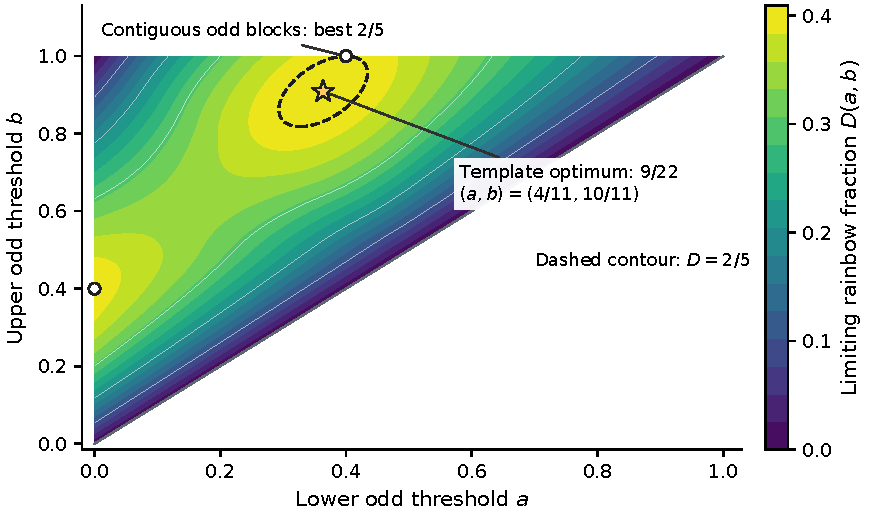
\includegraphics[width=.67\linewidth]{figures/schur_template_structure.pdf}
\caption{The two-threshold parity template has unique optimum $9/22$ at
$(a,b)=(4/11,10/11)$, compared with $2/5$ for a single contiguous odd block.
The analytic proof establishes the optimum throughout the stated domain;
the plot illustrates its dependence on the thresholds (generated using NumPy \citep{harris2020array}).}
\label{fig:schur-template-structure}
\end{figure}

\subsection{Cycle blowups: explaining the failure of recolorability}

The reconfiguration problem asks whether one proper coloring can be changed into another by recoloring one vertex at a time, keeping every intermediate coloring proper. To represent the allowed moves, the graph $R_k(G)$ has one vertex for each proper coloring of $G$ using colors from a set of size $k$, and an edge joins two colorings that differ at one vertex; a coloring may use fewer than $k$ of the available colors.

In these terms a graph is \emph{recolorable} if $R_k(G)$ is connected for every $k\ge\chi(G)+1$, where $\chi(G)$ is the chromatic number, and a \emph{frozen} coloring, one in which no vertex can change color without creating an equally colored adjacent pair, is an isolated vertex of $R_k(G)$.

In \emph{Recoloring via Modular Decomposition}, \citet{belavadi2026recoloring} ask whether recolorability of every induced subgraph of a prime graph guarantees recolorability of all its clique blowups; this is the preservation direction of their Conjecture~1, and the statement matches Section~6 of the originally reviewed arXiv~v2 input. Section~\ref{sec:mathematics} defines prime graphs and clique blowups; $C_n[K_2]$ replaces each cycle vertex by a two-vertex clique, with all edges between neighboring cliques.

The original counterexample uses $C_9$, which is prime and whose
induced subgraphs are all recolorable. Its blowup $C_9[K_2]$ has
chromatic number~5, but repeating the color pairs
$\{1,2\},\{3,4\},\{5,6\}$ around the cycle gives a frozen
six-coloring. Each vertex has neighbors using every alternative
color, so no first recoloring move is possible. A proper five-coloring
provides another vertex of the same reconfiguration graph, proving
that it is disconnected. Thus the blowup fails the conjecture's
conclusion even though the base graph satisfies its hypotheses.

\paragraph{Relation to fall colorings and the source construction.}
A frozen proper coloring is a fall coloring: every vertex sees all colors in its closed neighborhood~\citep{dunbar2000fall}.
For cycles, $3\in\operatorname{Fall}(C_n)$ exactly when $3\mid n$ \citep[Section~4]{lauri2019fall}.
Applying \citet[Theorem~2]{shaebani2009fall} with $G=C_n$, $H=K_2$, and three two-color palettes gives a fall six-coloring of $C_n[K_2]$ whenever $3\mid n$.
Shaebani also explicitly discusses $C_9[K_2]$ immediately after Corollary~3 and gives a fall five-coloring, so even this particular graph predates our recorded witness.
The source's Figure~3 displays the same periodic palettes on a doubled six-cycle; its base graph contains a non-recolorable induced $C_6$, so that example does not contradict Conjecture~1 \citep[Section~6]{belavadi2026recoloring}.
Our case uses this known construction at $n=9$ and verifies all the
hypotheses of the conjecture. In the follow-up, we used AI tools to
prove the odd-cycle characterization and labeled count below in Lean.
The cited constructions establish the existence direction; the
follow-up supplies the necessity and counting arguments. We report these
connections without asserting literature-wide priority for the
characterization or count.

The following proposition identifies exactly which odd-cycle blowups
have frozen six-colorings and counts them, showing that the original example is part of an
infinite family with exponentially many isolated colorings.

\begin{structuralproposition}[Frozen colorings in odd-cycle blowups]
\label{prop:cycle-blowup-frozen}
For every odd $n\ge5$, $C_n$ is prime and every induced subgraph is
recolorable. Its blowup $H_n=C_n[K_2]$ has chromatic number~5 and has
a frozen proper coloring with the six labeled colors $[6]$ if and only
if $3\mid n$. When $3\mid n$, there are exactly $90\cdot2^n$ frozen
labeled colorings, and $R_6(H_n)$ has at least $90\cdot2^n+1$ connected
components.
\end{structuralproposition}

The single $C_9[K_2]$ witness suggests looking at its repeated color
pairs. Call the pair assigned to each replacement clique its
\emph{palette}. The key is that the inability to recolor a vertex
imposes a local constraint on three neighboring palettes. In a frozen
coloring, every three consecutive two-vertex cliques must collectively
use all six colors. Overlapping triples of cliques therefore force
their palettes to repeat with period three. An ordered partition of the six
colors into pairs gives 90 choices; independently assigning each
clique's pair to its two labeled vertices gives $2^n$ choices.
Thus $C_{6r+3}[K_2]$, for every
$r\ge1$, is a counterexample to the same preservation claim. The
original $C_9[K_2]$ has 46,080 isolated six-colorings, not merely the
single exhibited state.

The witness thus becomes a classification: this six-color obstruction
occurs exactly at the odd multiples of three, and its multiplicity is known.
It persists for arbitrarily large prime base graphs while the blowups
keep chromatic number five. Clique substitution creates the obstruction
even though every induced subgraph of the base graph is recolorable.
This identifies what a repaired preservation theorem must address:
additional conditions on the substitution itself. The component count
is a lower bound. At the remaining odd lengths, determining connectivity
requires studying colorings that do admit individual moves.


\paragraph{Larger replacement cliques.}
The two-color palettes lead naturally to a further question: what
happens when each cycle vertex is replaced by a clique of size three?
For every natural $n\ge4$, the graph $C_n[K_3]$ has a frozen proper
eight-coloring exactly when
$8\lceil n/3\rceil\le3n$. This holds precisely for
$n\in\{6,8,9,11,12\}$ and all $n\ge14$.

The necessity argument tracks the cliques containing each color.
Those cliques form an independent dominating set of the base cycle:
no two are adjacent, and every other clique has a neighbor in the set.
For sufficiency, explicit sequences of palettes can be joined to cover
every allowed length. Three consecutive $K_3$ cliques have nine vertex
positions for eight colors, so a color can repeat in the two outer
cliques. This explains why the three-period argument for $K_2$ changes.
At $n=13$, the theorem rules out this particular obstruction; the
connectivity of the other colorings is a separate question.

Allowing the clique size to vary gives a broader construction. For
every odd $n\ge9$, taking $q=\lceil n/3\rceil$ yields a graph
$C_n[K_q]$ with chromatic number $2q+1<n$ and a frozen $n$-coloring.
Thus a suitable clique size removes the divisibility restriction on
the base cycle. We developed these later results with the help of AI
tools. Their graph statements are certified in
\path{mathematics/theorems/Q3Law.lean} and
\path{mathematics/theorems/AllOdd.lean};
\path{mathematics/index.json} records their exact scopes and build
receipts. Combining these graph statements with the source conjecture's
hypotheses is the written mathematical argument, rather than a single
additional Lean theorem linking all parts.

\subsection{Proofs of the structural counterexample propositions}
\label{app:counterexample-structural-proofs}

The rest of this appendix proves the two propositions above. The Schur proof counts rainbow triples, derives their limiting density, and optimizes the threshold pair; the cycle proof derives palette periodicity and counts the frozen colorings.

Both propositions also have Lean proofs under \path{mathematics/theorems/}, with statement and build records in \path{mathematics/index.json}: the Schur certificate connects finite counts to the limiting density and proves the family's unique optimum and sharp stability bound, and the cycle certificate covers every allowed cycle length. Finite checks of the original witnesses are supplied separately under \path{mathematics/discoveries/}.

\subsubsection{Schur template: counting, optimization, and stability}
\label{app:schur-template-proof}

\begin{proof}[Proof of Proposition~\ref{prop:schur-template-optimum}]
\textit{Count the two kinds of rainbow triple.}
Fix $0\le a\le b\le1$ and the coloring specified in the proposition.
Write $t=b-a$ for the width of the middle odd block and
$x_+=\max(x,0)$ for the positive part of $x$. The two odd color
classes have cardinalities $(1-t)n/2+O(1)$ and $tn/2+O(1)$.
There are $\binom n2$ ordered triples $x+y=z$ in $[n]$.

For each pair of differently colored odd integers, their positive even
difference yields exactly two mixed-parity rainbow triples, one for
each ordering of the addends. Conversely each mixed-parity rainbow
triple determines this pair. Their number is therefore
$t(1-t)n^2/2+O(n)$, contributing $t(1-t)$ to the limiting normalized
density.

For odd--odd addends, the sum is even and has color~1. Choose the
color-2 addend from $[0,a]\cup[b,1]$ and the color-3 addend from $[a,b]$
in normalized coordinates, subject to their sum being at most~1.
The lattice of odd pairs has density $n^2/4$ per unit area.
The factor two for ordering the addends and division by
$\binom n2\sim n^2/2$ cancel this factor $1/4$. Thus the limiting
contribution is the area of those two rectangles below the line
$x+y=1$. Boundary lattice squares number $O(n)$, giving an $O(n)$
error in the unnormalized count; this also justifies arbitrary real
thresholds and their rounding. Even--even addends cannot be rainbow.

For a rectangle $[u,v]\times[s,t]$, its area below $x+y=1$ is
\[
 \frac12\bigl[(1-u-s)_+^2-(1-v-s)_+^2
             -(1-u-t)_+^2+(1-v-t)_+^2\bigr].
\]
This follows by inclusion--exclusion from the triangle with lower
corner $(u,s)$. Applying the formula to the two rectangles gives
\begin{align}
 D(a,b)={}&(b-a)(1-b+a)\nonumber\\
 &+\frac12\bigl[(1-a)^2-(1-b)^2-(1-2a)_+^2
 -(1-2b)_+^2+2(1-a-b)_+^2\bigr].
 \label{eq:schur-template-objective}
\end{align}
In particular the limit exists.

\textit{Optimize the density over all threshold pairs.}
The allowed pairs form the triangle $0\le a\le b\le1$.
The lines $a=1/2$, $b=1/2$, and $a+b=1$ divide it into four regions. Expanding
Equation~\eqref{eq:schur-template-objective} gives the following
quadratics and Hessian determinants:
\begin{center}
\small
\begin{tabular}{p{0.26\linewidth}p{0.54\linewidth}r}
\toprule
Region & $D(a,b)$ & $\det\nabla^2D$ \\
\midrule
$0\le a\le b\le\tfrac12$
& $-\tfrac32a^2+4ab-\tfrac52b^2-2a+2b$ & $-1$ \\
$a\le\tfrac12\le b$, $a+b\le1$
& $-\tfrac32a^2+4ab-\tfrac12b^2-2a+\tfrac12$ & $-13$ \\
$a\le\tfrac12\le b$, $a+b\ge1$
& $-\tfrac52a^2+2ab-\tfrac32b^2+2b-\tfrac12$ & $11$ \\
$\tfrac12\le a\le b\le1$
& $-\tfrac12a^2+2ab-\tfrac32b^2-2a+2b$ & $-1$ \\
\bottomrule
\end{tabular}
\end{center}
The first, second, and fourth Hessians are indefinite. At an interior
local maximum a twice differentiable function must have negative
semidefinite Hessian, so these three regions attain their maxima on
their boundaries. In the third region the Hessian is
$\left(\begin{smallmatrix}-5&2\\2&-3\end{smallmatrix}\right)$,
which is negative definite. Its gradient vanishes uniquely at
$(a,b)=(4/11,10/11)$, strictly inside the region, with value $9/22$.

The following formulas cover every remaining boundary:
\begin{align*}
 D(a,a)&=0,\\
 D(0,b)&=\begin{cases}2b-\tfrac52b^2,&b\le\tfrac12,\\
                    (1-b^2)/2,&b\ge\tfrac12,\end{cases}\\
 D(a,1)&=\begin{cases}2a-\tfrac52a^2,&a\le\tfrac12,\\
                    (1-a^2)/2,&a\ge\tfrac12,\end{cases}\\
 D(a,\tfrac12)&=\tfrac38-\tfrac32a^2
                  &&(0\le a\le\tfrac12),\\
 D(\tfrac12,b)&=\tfrac38-\tfrac32(b-1)^2
                  &&(\tfrac12\le b\le1),\\
 D(a,1-a)&=3a-6a^2
                  &&(0\le a\le\tfrac12).
\end{align*}
The second and third lines have maximum $2/5$, attained at $b=2/5$
and $a=2/5$, respectively. Each of the final three has maximum $3/8$.
Thus every boundary value is at most $2/5<9/22$, proving the unique
global maximum over this template. The boundaries $a=0$ and $b=1$
are precisely the two contiguous odd-block subfamilies, proving their
claimed optima.

\textit{Measure the loss from moving the thresholds.}
Completing the square in the third region, with
$u=a-4/11$ and $v=b-10/11$, yields
Equation~\eqref{eq:schur-template-stability}. The loss matrix is
$\left(\begin{smallmatrix}5/2&-1\\-1&3/2\end{smallmatrix}\right)$
with eigenvalues $(4\pm\sqrt5)/2$, so in that region
\[
 \frac9{22}-D(a,b)\ge
 \frac{4-\sqrt5}{2}\left((a-\tfrac4{11})^2+(b-\tfrac{10}{11})^2\right).
\]
This inequality quantifies stability within the template: the loss
in density is at least a fixed positive multiple of the squared distance
from the optimal threshold pair. The wider problem allows arbitrary
three-colorings and requires a separate upper bound.
\end{proof}

The public file \path{mathematics/theorems/SchurTemplateComposed.lean}
contains the counting, limit, and optimization arguments. It checks
Equation~\eqref{eq:schur-template-objective}, including every boundary,
using nonnegative polynomial decompositions in the four regions.
For the sharp coefficient, writing $s=(1+\sqrt5)/2$,
$\lambda=(4-\sqrt5)/2$, and
$Q(u,v)=5u^2/2-2uv+3v^2/2$, it verifies
$s[Q(u,v)-\lambda(u^2+v^2)]=(su-v)^2$.
Equality therefore holds exactly on $v=su$. Any nonzero vector on
that line proves that the coefficient cannot be increased for this
quadratic form.

The corresponding declarations are
\path{CoPEER.SchurTemplate.unique_global_optimum},
\path{sharp_stability}, \path{quadratic_spectral_equality_iff}, and
\path{quadratic_spectral_coefficient_optimal}.
The declaration \path{paper_limit} proves the counting and limit
correspondence preceding Equation~\eqref{eq:schur-template-objective};
the composed theorem joins it to the optimization result.
\path{mathematics/builds/schur.json} records the compiled
source and log hashes.

\subsubsection{Odd-cycle blowups: palette periodicity and component counts}
\label{app:cycle-blowup-proof}

\begin{proof}[Proof of Proposition~\ref{prop:cycle-blowup-frozen}]
\textit{Verify the conjecture's hypotheses for the base cycle.}
A graph is $d$-degenerate if every nonempty induced subgraph has a
vertex of degree at most $d$. The standard degeneracy recoloring
argument \citep{cereceda2008connectedness} shows that if a finite graph
$X$ is $d$-degenerate, then $R_k(X)$ is connected for every $k\ge d+2$.
Here vertices of $R_k(X)$ are proper maps $V(X)\to[k]$, without
requiring surjectivity, and an edge changes one vertex's color.
To prove the lemma, induct on $|V(X)|$. Remove a vertex $v$ of degree
at most $d$, and connect the restrictions of any two colorings by
induction. Lift that path to $X$. If a neighbor is about to acquire
the current color of $v$, first move $v$ to a different color absent
from its neighborhood; at least two colors are absent because
$k\ge d+2$. Then perform the neighbor's move. Finally give $v$ its
target color. This proves connectivity for all required $k$.

For $n\ge5$, $C_n$ is prime. To see this, a \emph{module} is a set of
vertices that all have the same neighbors outside the set. A proper
module $S$ with at least two vertices would, by connectivity, have an outside vertex
$v$ adjacent to a member of $S$. Modularity makes $v$ adjacent to
every member of $S$, so degree two forces $S=N(v)$. The other
neighbor of either member of $S$ lies outside $S$ and distinguishes
its two members, a contradiction. For odd $n$, $C_n$ has chromatic
number three and degeneracy two, so the lemma proves recolorability
for every $k\ge4$. Each proper induced subgraph is a disjoint union
of paths. With an edge it has chromatic number two and degeneracy
one, so the lemma applies for every $k\ge3$. Nonempty edgeless
graphs recolor one vertex at a time for every $k\ge2$; the empty
graph has one coloring. Thus all induced subgraphs satisfy the full
definition of recolorability.

\textit{Determine the chromatic number of the blowup.}
Call each replacement clique a \emph{bag}, and index the bags of
$H_n=C_n[K_2]$ cyclically by $0,\ldots,n-1$. An independent set takes at most one vertex per
bag, and its occupied bags form an independent set of $C_n$.
Conversely every such set of bags lifts to an independent set.
Therefore $\alpha(H_n)=(n-1)/2$, and for odd $n\ge5$,
\[
 \chi(H_n)\ge\left\lceil\frac{2n}{(n-1)/2}\right\rceil
 =\left\lceil\frac{4n}{n-1}\right\rceil=5.
\]
For the matching upper bound, give the first $n-3$ bags alternating
palettes $\{1,2\},\{3,4\}$. The prefix length is even, so its last
palette is $\{3,4\}$. Give the last three bags, in order,
$\{1,5\},\{2,3\},\{4,5\}$. Adjacent palettes, including the last
and first, are disjoint. Assign each palette's two colors once in
its bag. This is a proper five-coloring for every specified $n$.

\textit{Identify exactly when a coloring is frozen.}
In any proper six-coloring, write $P_i$ for the two-element palette
on bag $i$. Every vertex of $H_n$ has degree five, and its closed
neighborhood consists exactly of the six vertices in bags
$i-1,i,i+1$. It cannot change color precisely when its five
neighbors use all five alternative colors. The coloring is
therefore frozen if and only if, for every $i$, the palettes
$P_{i-1},P_i,P_{i+1}$ are pairwise disjoint and partition $[6]$.
Comparing this partition with that for $i+1$ forces
$P_{i-1}=P_{i+2}$: both are the complement of $P_i\cup P_{i+1}$.
Hence the palettes have period three. If $3\nmid n$, then
$\gcd(3,n)=1$, so this periodicity around the cycle makes all
palettes equal, contradicting adjacent disjointness. If $3\mid n$,
any ordered partition of $[6]$ into three pairs, repeated around
the cycle, supplies a frozen coloring.

\textit{Count the isolated colorings.}
There are $6!/(2!)^3=90$ ordered partitions for bags $0,1,2$.
Each determines all other palettes, and in each labeled bag we can assign the
two colors to its two labeled vertices in two
ways, independently. The exact frozen-coloring count is thus
$90\cdot2^n$. Each is an isolated vertex of $R_6(H_n)$. The explicit
five-coloring, regarded as a six-coloring, has unused color~6, so
any vertex can move to that color. It lies in a further component,
giving at least $90\cdot2^n+1$ components. For odd $n$ divisible by
three, write $n=6r+3$ with $r\ge1$. These graphs refute the same
prime-blowup preservation claim at $6=\chi(H_n)+1$.
\end{proof}

The exact count distinguishes vertex labels and color labels, just as
$R_k$ does. It gives a lower bound on the number of connected components:
each frozen coloring contributes one, and the five-coloring contributes
another. For $3\nmid n$, deciding connectivity requires examining the
components formed by colorings that can make single-vertex moves.
